\documentclass[12pt]{article}
\usepackage[utf8]{inputenc}
\usepackage[english]{babel}
\usepackage[table,xcdraw]{xcolor}
\usepackage{hyperref}
\usepackage{float}
\usepackage{amsmath}
\usepackage{mathtools}
\usepackage{tikz}
\usepackage{pgfplots}
\usepackage{blindtext}

\pgfplotsset{compat=1.14} % Disable-lint

\hypersetup{%
	colorlinks,
	citecolor=black,
	filecolor=black,
	linkcolor=black,
	urlcolor=black
}

\usepackage[backend=biber,style=authoryear]{biblatex}
\usepackage[newfloat]{minted}
\usemintedstyle{vs}
\usepackage{csquotes}
\usepackage{caption}
\usepackage{booktabs}


\graphicspath{ {images/} }

\newcommand\tab[1][1cm]{\hspace*{#1}}
\SetupFloatingEnvironment{listing}{name=Code example}
\definecolor{bg}{rgb}{0.95,0.95,0.95}
\newenvironment{code}{\captionsetup{type=listing}}{}

\newcommand\codeblock[3]{%
\begin{code}
	\caption{#3}
	\inputminted[%
	    mathescape,
	    linenos,
	    numbersep=5pt,
	    tabsize=4,
	    label=Helloworld,
	    bgcolor=bg,
	    breaklines%
	]{TypeScript}{#1}
\label{#2}
\end{code}
}

\newcommand\Code[1]{\texttt{#1}}


\usepackage{dirtree}

\addbibresource{references.bib}

\begin{document}

\begin{titlepage}
	\centering
	\vspace{2cm}
	{\Huge Software implementations and analysis of three voting systems\par}
	\vspace{0.6cm}
	{\LARGE Adrian Salamon\par}
	\vspace{0.6cm}
	{\Large Kungsholmens gymnasium\par}
	\vspace{0.4cm}
	{\large Senior thesis\par}
	\vspace{0.6cm}
	
\includegraphics[width=0.3\textwidth]{kg}\par\vspace{1cm}
	\vspace{4cm}
	\vfill
	Supervised by: \par
	Maja Kankaanranta

	\vfill

	% Bottom of the page
	{\large \today\par}
\end{titlepage}


\pagebreak




\begin{abstract}
\end{abstract}

\pagebreak

\tableofcontents

\pagebreak

\section{Introduction}
\subsection{Background}
Taking a collective decision as a population is difficult. To solve this issue, various voting systems with defined rules are used. They are used to show common preferences within a population, for example what politician a population wants to see elected. Several types of systems have been designed for this purpose and there are a myriad of variations of those systems. They range from simple methods such as “most votes win” to complex processes that can only be practically carried out by a computer. However, practically all voting systems are algorithmic in nature, which makes them interesting to study for both Computer Scientists and Mathematicians. When deciding on what systems that shall be used, it is useful to know what differences and similarities they have.
\subsection{Purpose}
The purpose of this essay is to evaluate differences and similarities in terms of election results in three different voting systems: Single Transferable Vote (STV), First-Past-The-Post (FPTP) and the Schulze Method. This paper will only be examining and discussing differences and similarities in the results of the methods, not touching on how practically feasible the methods might be in actual elections.
\pagebreak
\section{Theory}
One would think that by testing all different voting systems and by setting up good criteria for how to evaluate them, it would be possible to come to a definitive conclusion of what system should be used. However, this is not the case. By setting up different mathematical criteria for how a voting system shall behave, it is impossible to satisfy all criteria simultaneously. This is what several theorems, most notably \textit{Arrow's Impossibility Theorem} show \autocite{arrow1950difficulty}. This means that any decision regarding choice of electoral system is a balance of their strengths and weaknesses. Simply put: there is no perfect voting system and never will be. This does, however, not mean that all voting systems are equally efficient, elegant or accurate.

There are several ways of evaluating voting methods. One is the mathematical approach of evaluating what criteria are important to meet and finding methods that satisfy them. Another is by testing and finding probabilities that some criteria are broken — A method that fails to meet a certain criterion only in very few cases is perhaps not a big problem. A third way of evaluating methods is not by mathematical criteria, but other metrics such as voter satisfaction or how likely someone is to vote tactically.
\subsection{Definitions}
\begin{itemize}
	\item A \textit{candidate} is someone a voter can vote for to elect. It can also be considered as being a party that a voter can vote for.
	\item An \textit{election} is an event in which voters cast ballots to vote for candidates
	\item A \textit{seat} is something a candidate can be elected to. A candidate may for example be elected to hold a seat of parliament.
	\item An \textit{ideology} is a group that both candidates and voters can identify with. They split the whole voting population into several blocks. Several candidates can belong to one ideology.
\end{itemize}  
\pagebreak
\section{Methodology}
All voting algorithms have been implemented in Typescript – mostly due to the author having previous experience with JavaScript. Typescript is a superset of JavaScript with multiple extra features. Most importantly, Typescript has optional static type checking. Sample code written in Typescript can be seen in code example~\ref{lst:typescript example}.
\codeblock{code/typescriptexample.ts}{lst:typescript example}{Basic Typescript syntax}
\subsection{Modeling test data}
\label{sec:vote-generation}
In order to test the methods and their implementations, test data is needed. There are cases where extensive election data is published, such as in Maltese elections, but full ballot data, which is needed as input for the implementations used in this paper has not been found. Instead, the algorithms will be tested with data generated from a simple ballot-generating computer program. The program used for this purpose in this paper is highly primitive, as modeling preferences within a population is far beyond the scope of this paper. The full ballot generation program can be found in the \Code{/generator} folder. The goal of the program is to produce ballots that rank every candidate in order of preference (see figure~\ref{fig:stv ballot} on page~\pageref{fig:stv ballot}). The program incorporates the idea of an \textit{ideology} where each candidate is assigned one. Each ideology has has a list of weighted preferences indicating how a voter for this ideology is likely to vote. The weighed preferences are generated via an abstraction. A single configuration object is used to create all ideologies.
\codeblock{code/generator/ideologyConfig.ts}{lst:ideology configuration}{Configuration object for creating ideologies}
The program then works via 4 major steps:
\begin{enumerate}
	\item It assigns each candidate to an ideology based on the size of the ideology. A larger ideology has more candidates.
	\item It creates a base ``strength'' to each candidate. Within each ideology, every candidate is assigned its relative strength. The relative strength is generated by a negative exponential function with a different constant (based on the \Code{candidatePower}). The strength of each candidate is then multiplied by the size of their ideology and then normalized. This gives a base strength of all candidates. This simulates the probability for vote from a non-ideological voter for a particular candidate.
	\item Based on the base strength of each candidate, a probability distribution of votes for each candidate is created for each ideology. This process takes  the  \Code{ideologyPower} constant into account. An ideology's probability distribution represents how a voter aligned with the ideology is likely to vote. A strong ideology may thus attract votes from voters aligned with another ideology.
	\item It creates a certain number of individual ballots. Each ballot is given an ideology and based on the probability distribution of that particular ideology, it creates its own list of preferences for candidates. This is done via weighed random number generation.
\end{enumerate}
The output of the program is a set of ballots, where each ballot is an ordered set of preferences between candidates. The implementation is highly arbitrary and as are all constants. However, expanding on the generator program would be beyond the scope of this project. The vote generation algorithm is an attempt to provide more realistic voting data than what is achieved by a purely random allocation of votes. The program also allows for the possibility to control the data by changing the input variables. This makes it possible to test different election scenarios.
\subsection{Constructing test scenarios}
Constructing test scenarios, ie.\ election conditions, is difficult task. Due to there being so many variables both in real elections and the simulated elections in the generator program, it makes it practically impossible to control for all variables. Instead, 3 arbitrary test scenarios will be used. An election will be run 1000 times for each scenario and the election data will then processed by each voting algorithm and the results will be compared. The three simulation scenarios are arbitrary but should allow for comparison of the different voting methods. All simulations will have three ideologies and 500 ballots.
\subsubsection{Scenario 1}
\label{sec:method-scenario1}
The scenario is built around electing one candidate out of eight. The spread of votes within ideologies is ``flat'' and all ideologies are so called ``weak''. This means that the general spread of votes between candidates will be even. An example of the distribution of first-preference votes generated in this scenario can be seen in figure~\ref{fig:example of scenario 1}. The full configuration object can be seen in code example~\ref{lst:scenario 1}.
\codeblock{code/generator/scenario1.ts}{lst:scenario 1}{Configuration object for scenario 1}
\begin{figure}[H]
	\centering
	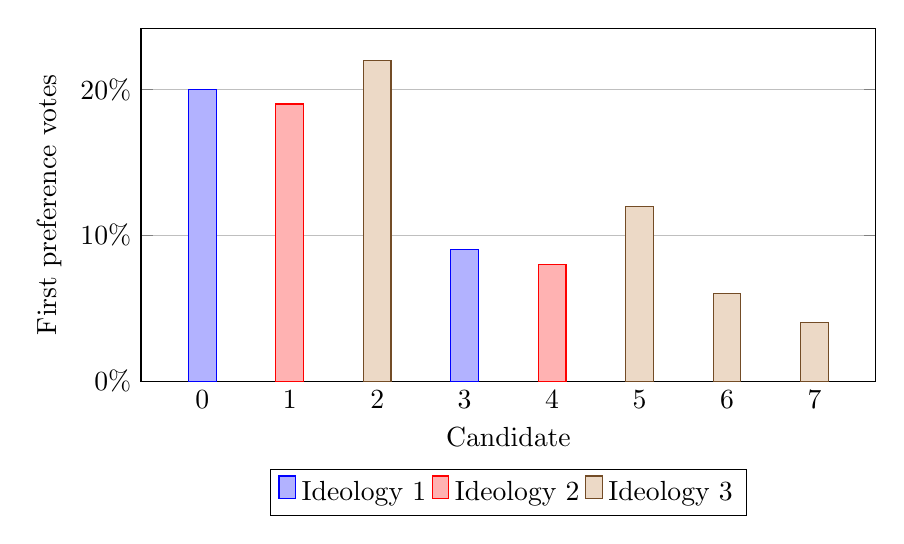
\begin{tikzpicture}
		\begin{axis}[
			ybar stacked,
			width = 0.9\textwidth,
			height = 0.5\textwidth,
			legend style={at={(0.5,-0.25)},
			anchor=north,legend columns=-1},
      x tick style = transparent,
			ylabel = {First preference votes},
			xlabel = {Candidate},
			ymajorgrids = true,
      ymin = 0,
			yticklabel={\pgfmathprintnumber\tick\%}
      ]
			\addplot coordinates
			{(0, 20)(1, 0)(2, 0)(3, 9)(4, 0)(5, 0)(6, 0)(7, 0)};
			\addplot coordinates
			{(0, 0)(1, 19)(2, 0)(3, 0)(4, 8)(5, 0)(6, 0)(7, 0)};
			\addplot coordinates
			{(0, 0)(1, 0)(2, 22)(3, 0)(4, 0)(5, 12)(6, 6)(7, 4)};
			\legend{Ideology 1, Ideology 2, Ideology 3}
		\end{axis}
	\end{tikzpicture}
	\caption{Example distribution of first-preference votes in scenario 1. Avreages of 10 simulations.}
\label{fig:example of scenario 1}
\end{figure}
\subsubsection{Scenario 2}
\label{sec:method-scenario2}
The second scenario elects 3 candidates out of 9 total. The parameters are set to produce a ``normal'' spread of votes between candidates. An example distribution of first-preference votes generated in this scenario can be seen in figure~\ref{fig:example of scenario 2}. The full configuration can be seen in code example~\ref{lst:scenario 2}.
\codeblock{code/generator/scenario2.ts}{lst:scenario 2}{Scenario 2}
\begin{figure}[H]
	\centering
	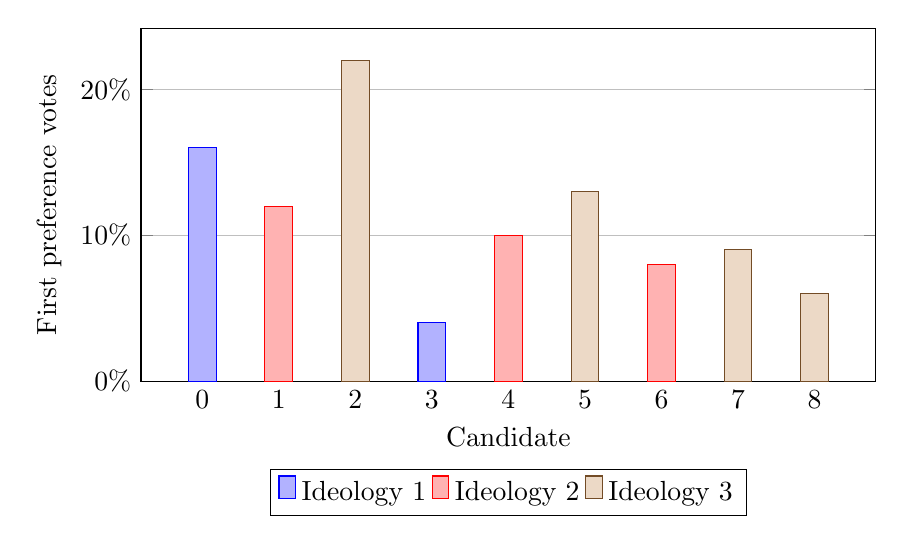
\begin{tikzpicture}
		\begin{axis}[
			ybar stacked,
			width = 0.9\textwidth,
			height = 0.5\textwidth,
			legend style={at={(0.5,-0.25)},
			anchor=north,legend columns=-1},
      x tick style = transparent,
			ylabel = {First preference votes},
			xlabel = {Candidate},
			ymajorgrids = true,
      ymin = 0,
			yticklabel={\pgfmathprintnumber\tick\%}
      ]
			\addplot coordinates
			{(0, 16)(1, 0)(2, 0)(3, 4)(4, 0)(5, 0)(6, 0)(7, 0)(8, 0)};
			\addplot coordinates
			{(0, 0)(1, 12)(2, 0)(3, 0)(4, 10)(5, 0)(6, 8)(7, 0)(8, 0)};
			\addplot coordinates
			{(0, 0)(1, 0)(2, 22)(3, 0)(4, 0)(5, 13)(6, 0)(7, 9)(8, 6)};
			\legend{Ideology 1, Ideology 2, Ideology 3}
		\end{axis}
	\end{tikzpicture}
	\caption{Example distribution of first-preference votes in scenario 2. Avreages of 10 simulations.}
\label{fig:example of scenario 2}
\end{figure}
\subsubsection{Scenario 3}
\label{sec:method-scenario3}
The second scenario elects 3 candidates out of 9 total. It features a steep spread of votes between candidates. An example distribution of first-preference votes generated in this scenario can be seen in figure~\ref{fig:example of scenario 3}. The full configuration can be seen in code example~\ref{lst:scenario 3}.
\codeblock{code/generator/scenario3.ts}{lst:scenario 3}{Scenario 3}
\begin{figure}[H]
	\centering
	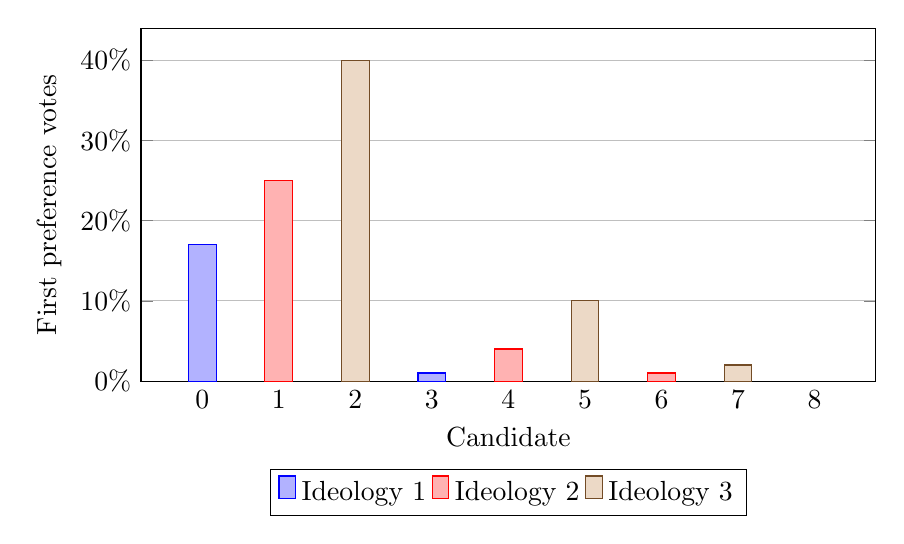
\begin{tikzpicture}
		\begin{axis}[
			ybar stacked,
			width = 0.9\textwidth,
			height = 0.5\textwidth,
			legend style={at={(0.5,-0.25)},
			anchor=north,legend columns=-1},
      x tick style = transparent,
			ylabel = {First preference votes},
			xlabel = {Candidate},
			ymajorgrids = true,
      ymin = 0,
			yticklabel={\pgfmathprintnumber\tick\%}
      ]
			\addplot coordinates
			{(0, 17)(1, 0)(2, 0)(3, 1)(4, 0)(5, 0)(6, 0)(7, 0)(8, 0)};
			\addplot coordinates
			{(0, 0)(1, 25)(2, 0)(3, 0)(4, 4)(5, 0)(6, 1)(7, 0)(8, 0)};
			\addplot coordinates
			{(0, 0)(1, 0)(2, 40)(3, 0)(4, 0)(5, 10)(6, 0)(7, 2)(8, 0)};
			\legend{Ideology 1, Ideology 2, Ideology 3}
		\end{axis}
	\end{tikzpicture}
	\caption{Example distribution of first-preference votes in scenario 3. Avreages of 10 simulations.}
\label{fig:example of scenario 3}
\end{figure}
\subsection{Metrics for evaluating results}
Three metrics will be used for comparing the results obtained in the different scenarios. The results obtained with each voting method will be compared against the other methods. Comparisons to the configuration files outlined in Sections~\ref{sec:method-scenario1} -~\ref{sec:method-scenario3} will also be made.
\subsubsection{Standard deviation}
The standard deviation of the outcomes represents the variance in outcome due to the pseudorandom nature of the generator program outlined in Section~\ref{sec:vote-generation}. The standard deviation is calculated according to equation~\ref{eq:standard-deviation}. 
\begin{equation}
	\label{eq:standard-deviation}
	\sigma ={\sqrt {{\frac {1}{N}}\sum _{i=1}^{N}(x_{i}-\mu )^{2}}},{\rm {\ \ where\ \ }}\mu ={\frac {1}{N}}\sum _{i=1}^{N}x_{i}.
\end{equation}
\subsubsection{Misrepresentation}
The misrepresentation metric gives an idea of how \textit{proportional} the outcomes of a certain voting method in any scenario is. The level of proportionality of a result is a measure of how closely the preferences of a population in terms of ideology are matched with the result. Higher proportionality means that the election outcome more closely resembles the ideological preferences of the voters. The method of calculating the misrepresentation used in this paper is defined as follows:
\begin{enumerate}
	\item Calculate what theoretical election outcome would be the most proportionate in terms of ideology based on the configuration file used to generate the ballots.\label{enum:theoretical}
	\item Compare the actual outcomes of a certain method with the theoretical result obtained in Step~\ref{enum:theoretical}.
	\begin{enumerate}
		\item Calculate the difference between the measured and theoretical percentage for each ideology.
		\item Sum all the differences.
	\end{enumerate}
\end{enumerate}
\subsubsection{Most likely winners}
Shows what candidates, given a certain scenario, are most likely to win in a particular method.
\pagebreak
\section{Specification of voting methods}
\subsection{First-past-the-post}
\subsubsection{Description}
The first-past-the-post voting method is a method designed for electing one or several (N) candidates out of a set of candidates. Each voter has one vote that may be allocated to any candidate. In a FPTP election the N candidates with most votes get elected.
\subsubsection{Justification}
The method is simple and can easily be understood. The first-past-the-post method is widely used in for example the United Kingdom and United States. Comparisons with this method can also easily be made.
\subsubsection{Pseudocode}
let $V$ be the set of votes with $V_{i}$ being the number of votes for candidate $i$ \\
let $N$ be number of candidates to be elected \\
sort $V$ based on $V_{i}$\\
slice $V$ between $0$ and $N$
\subsubsection{Implementation}
The first-past-the-post program is implemented in a single file (\Code{/fptp/index.ts}). The inputs of the program can be seen in code example~\ref{lst:fptp inputs}.
\codeblock{code/fptp/inputs.ts}{lst:fptp inputs}{Inputs for FPTP program}
The program sums all the first-preference votes for each candidate and elects the ones with most votes, in accordance with specified amount of seats.
\subsection{Single transferable vote}
\subsubsection{Description}
The Single Transferable Vote (STV) is a more complicated voting system than the first-past-the-post method. STV is a multi-seat election method, although it can be used for single-seat elections too. STV becomes equivalent to the Instant-runoff voting method (IRV) in single-seat elections. In an STV election, voters are given ballots in which they are supposed to rank candidates in order. The specific rules for wether one needs to rank all candidates or just a few can vary. For the sake of simplicity, all candidates must be ranked at unique and linear values in this implementation. An example of an STV ballot can be seen in figure~\ref{fig:stv ballot}. By having voters convey more information in a ballot, there is more data available that the method can take advantage of. 
\begin{figure}
	\centering
	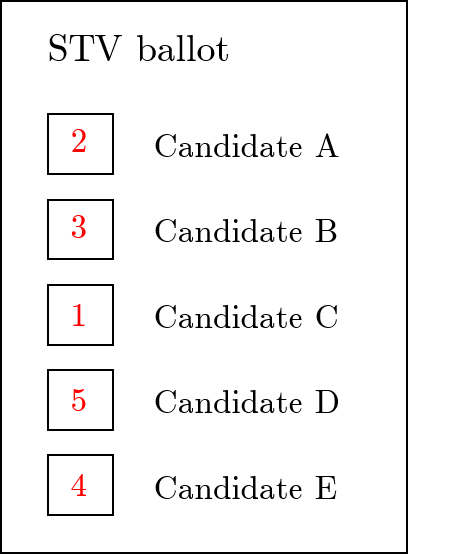
\includegraphics[height=140px]{ballot}
	\caption{Sample STV ballot}
\label{fig:stv ballot}
\end{figure}

Using this data, votes are transferred between candidates within a ballot, hence the name Single Transferable Vote. The method relies on the concept of a quota, which is the number of votes one needs to be elected. The Droop-Quota, defined as $(\frac{\text{total valid poll}}{\text{seats} + 1})+1$, is often used and is the one implemented in this paper. If a candidate receives equal or more votes than the quota, he/she is elected. If the number of votes for a candidate exceed the quota, a fraction of his/her votes are transferred to the next choice on the ballots that voted for that particular candidate. This process is repeated until there are no candidates with more votes than the quota. If there still are seats yet to be filled, the candidate with fewest votes is eliminated and his/her votes are transferred to the next choice on the ballots which supported the candidate. This process is repeated until all seats are filled. The process can become quite complex with many ballots and transferring of fractional votes. A computer is therefore essential to resolve large scale elections.
\subsubsection{Justification}
STV is an established voting method in use in several countries. It is used for parliamentary elections in Ireland, Malta and Australia as well as being used in local and regional elections across the world.
\subsubsection{Pseudocode}
\label{alg:stv psuedocode}
let $quota$ be the quota \\
let $seats$ be the number of seats \\
let $winners$ be the list of elected candidates \\
let $votes$ be the set of votes with $votes_{i}$ signifying votes for candidate $i$\\
while $\left\vert{winners}\right\vert < seats$\\
\tab if any candidate $i \notin winners$ and $votes_{i} \geq quota$ \\
\tab\tab add $i$ to $winners$ \\
\tab\tab continue \\
\tab end if \\
\tab if any candidate $i$ where $votes_{i} > quota$\\
\tab\tab multiply $votes_{i}$ with $(1 - \frac{\text{surplus votes}_{i}}{votes_{i}})$ \\
\tab\tab multiply next preferences for $votes_{i}$ with $\frac{\text{surplus votes}_{i}}{votes_{i}}$ and \\ \tab\tab distribute into $votes$\\
\tab\tab continue \\
\tab end if \\
\tab if $\left\vert{votes}\right\vert = seats$ \\
\tab\tab add all $votes \notin winners$ to $winners$ \\
\tab\tab continue \\
\tab end if \\
\tab $k \coloneqq$ index of smallest $votes_{i}$ \\
\tab eliminate $votes_{k}$ and distribute all next-preference votes for candidate \\
\tab $k$ into $votes$\\
end while
\subsubsection{Implementation}
The STV algorithm uses a tree structure to represent the state of the election. Every candidate is a top-level node with an attribute showing the number of current votes for the candidate. Each node has child nodes representing the next preferences of the voters for that particular candidate, see figure~\ref{fig:tree structure}. It is easy to manipulate branches via recursive functions. Merging and multiplying branches is used when transferring votes from one candidate node to another. A candidate node is a Typescript class. It can be found in the \Code{stv/candidate.ts} file and has the following properties and functions:
\begin{figure}
	\centering
	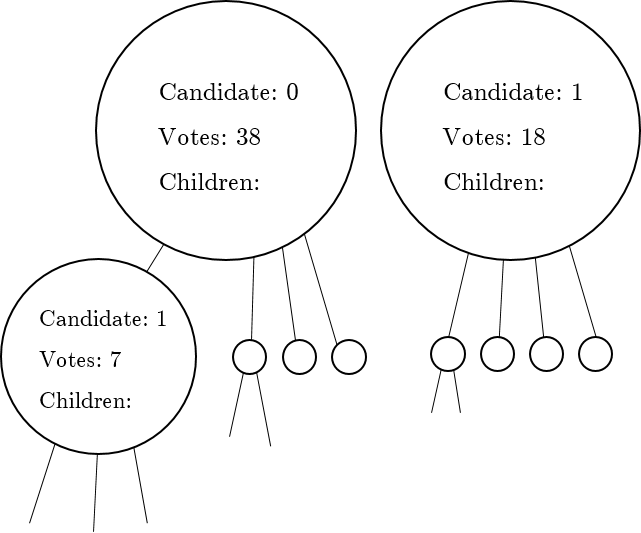
\includegraphics[height=200px]{Tree}
	\caption{Simplified and shortened version of the tree structure. Each candidate is a top-level node with children, signifying the preferences of the voters for that candidate.}
\label{fig:tree structure}
\end{figure}
\codeblock{code/stv/candidateNode.ts}{lst:stv candidate node}{The CandidateNode class}
With the \Code{add()} and \Code{multiply()} functions it is possible to recursively modify branches. There are two different manipulations that need to be preformed on the tree: transferring surplus votes and eliminating candidates. Both functions rely on the \Code{distribute()} function which is used to distribute a set of nodes onto the tree.
\codeblock{code/stv/distribute.ts}{lst:stv distribute function}{The distribute function}
In order to eliminate and transfer surplus votes from any candidate node $A$, the children of $A$ are passed into the distribute function. In the case of transferring surplus votes, the votes for each child node is first multiplied by $\frac{\text{surplus votes}}{\text{total votes}}$ as outlined in the pseudocode in Section~\ref{alg:stv psuedocode}. The full source code for functions that manipulate the tree structure can be found in \Code{/stv/tree.ts}.
The main process of the program is found in the \Code{stv/election.ts} file and runs the process defined in the pseudocode in Section~\ref{alg:stv psuedocode} on page~\pageref{alg:stv psuedocode}.
\subsection{Schulze}
\subsubsection{Description}
The Schulze Method is a method used mainly to determine results in single-winner elections but can also be used to provide rankings and elect multiple candidates in a single election \autocite{Schulze2011}. Ballots are identical to those of the Single Transferable Vote (see figure~\ref{fig:stv ballot} on page~\pageref{fig:stv ballot}). The method is compliant with the Condorcet Criterion, which means that if there is a candidate who the majority prefers in a pairwise comparison with every other candidate, that candidate wins. As mentioned, this method relies on comparing the preferences of every candidate to one another as shown in table~\ref{tab:pairwise comparison matrix}. If there is a Condorcet winner the process is simple: declare the Condorcet winner a winner and run another iteration without that candidate. Repeat this process until all seats are filled. However, there can be Condorcet ties, where there is no Condorcet winner. There are multiple methods used for resolving Condorcet ties, with one of them being the Schulze Method.

The Schulze Method resolves ties by investigating possible paths between candidates. For example, if out of a total of 50 ballots 30 ballots prefer $B>A$, 28 ballots prefer $A>C$ and 27 ballots prefer $C>B$, a path from $A$ to $B$ can be created by going $A \rightarrow C \rightarrow B$. The path is said to have the $strength$ of the weakest link in the path. In this example, the path strength between A and B is 27 due to the link between $C$ and $B$ having a strength of 27. There may be several paths between two candidates and the goal of the process is to find the strongest path between any candidate $A$ and $B$, written as $p[A,B]$. By finding the strongest path between all nodes a result can be obtained where $p[X,Y] \geq p[Y,X]$ which means that candidate $X$ wins. The Schulze Method also provides a linear ranking between all candidates, for example that $E > B > A > C > D$. By selecting the $N$ top candidates one can use the method for a multi-seat election. As the process can become very complex as the number of candidates grow, a computer is needed to resolve large elections.

The difficult problem in this method is finding the strongest path between candidates. The problem is called the widest path problem in graph theory. An efficient and relatively simple way to compute this problem is via the Floyd-Warshall algorithm which is used in the implementation. See Code Example~\ref{lst:schulze algorithm} for the full algorithm.

\begin{table}
\centering
\caption{Pairwise comparison matrix used in the Schulze method. For example, 17 ballots prefer $A>B$ and 33 ballots prefer $B>A$.}
\begin{tabular}{l|c|c|c|c|c|}
\cline{2-6}
 & \multicolumn{1}{l|}{A} & \multicolumn{1}{l|}{B} & \multicolumn{1}{l|}{C} & \multicolumn{1}{l|}{D} & \multicolumn{1}{l|}{E} \\ \hline
\multicolumn{1}{|l|}{A} & \cellcolor[HTML]{9B9B9B} & \cellcolor[HTML]{FFDDDD}17 & \cellcolor[HTML]{FFDDDD}14 & \cellcolor[HTML]{DDFFDD}35 & \cellcolor[HTML]{DDFFDD}30 \\ \hline
\multicolumn{1}{|l|}{B} & \cellcolor[HTML]{DDFFDD}33 & \cellcolor[HTML]{9B9B9B} & \cellcolor[HTML]{FFDDDD}24 & \cellcolor[HTML]{DDFFDD}47 & \cellcolor[HTML]{DDFFDD}36 \\ \hline
\multicolumn{1}{|l|}{C} & \cellcolor[HTML]{DDFFDD}36 & \cellcolor[HTML]{DDFFDD}26 & \cellcolor[HTML]{9B9B9B} & \cellcolor[HTML]{DDFFDD}40 & \cellcolor[HTML]{DDFFDD}42 \\ \hline
\multicolumn{1}{|l|}{D} & \cellcolor[HTML]{FFDDDD}15 & \cellcolor[HTML]{FFDDDD}3 & \cellcolor[HTML]{FFDDDD}10 & \cellcolor[HTML]{9B9B9B} & \cellcolor[HTML]{FFDDDD}18 \\ \hline
\multicolumn{1}{|l|}{E} & \cellcolor[HTML]{FFDDDD}20 & \cellcolor[HTML]{FFDDDD}14 & \cellcolor[HTML]{FFDDDD}8 & \cellcolor[HTML]{DDFFDD}32 & \cellcolor[HTML]{9B9B9B} \\ \hline
\end{tabular}
\label{tab:pairwise comparison matrix}
\end{table}
\subsubsection{Justification}
The Schulze method is used by multiple organizations around the world. It has been used by various software organizations such as The Wikimedia Foundation, The Debian Project and Ubuntu. It is also used by political parties such as the Pirate Party in Sweden and various other countries. The process also differs greatly in both method and implementation from the two other voting methods used in this paper.
\subsubsection{Pseudocode}
\label{alg:schulze psuedocode}
let $d[i,j]$ be the number of ballots that prefer candidate $i$ to candidate $j$\\
let $p[i,j]$ be the strength of the strongest path from candidate $i$ to candidate $j$\\
let $C$ be the number of candidates
for $i$ from 1 to $C$\\
\tab for $j$ from 1 to $C$\\
\tab\tab if ($i \ne j$)\\
\tab\tab\tab if ($d[i,j] > d[j,i]$)\\
\tab\tab\tab\tab $p[i,j] \coloneqq d[i,j]$\\
\tab\tab\tab else\\
\tab\tab\tab\tab $p[i,j] \coloneqq 0$\\
\tab\tab\tab end if \\
\tab\tab end if \\
\tab end for \\
end for\\
for $i$ from 1 to $C$\\
\tab for $j$ from 1 to $C$\\
\tab\tab if ($i \ne j$)\\
\tab\tab\tab for $k$ from 1 to $C$\\
\tab\tab\tab\tab if ($i \ne k \text{ and } j \ne k$)\\
\tab\tab\tab\tab\tab $p[j,k] \coloneqq \text{max }(p[j,k], \text{ min }(p[j,k], p[i,k]))$\\
\tab\tab\tab\tab end if \\
\tab\tab\tab end for \\
\tab\tab end if \\
\tab end for \\
end for\\
\subsubsection{Implementation}
The Schulze Method is implemented within the file \Code{schulze/index.ts}. It takes two inputs: a list of ballots and the number of seats to be elected. A ballot is an ordered list of candidates. The output of the program is a list of winners. The program first creates the matrices for both the preferences and paths between candidates as seen in Code Example~\ref{lst:schulze-maps}.
\codeblock{code/schulze/maps.ts}{lst:schulze-maps}{Data representation}
The program then runs the algorithm outlined in the pseudocode in Section~\ref{alg:schulze psuedocode}.
\codeblock{code/schulze/algorithm.ts}{lst:schulze algorithm}{Main algorithm}
\section{Evaluation of results}
\subsection{Scenario 1}
\label{sec:resuls-scenario1}
Scenario 1 featured eight candidates where one was to be elected. Vote spread was flat, meaning that votes tended to be diverse in their preferences. This means that there is not an obvious winner present. This can be seen from the first-preference votes in the scenario seen in figure~\ref{fig:example of scenario 1} on Page~\pageref{fig:example of scenario 1}. The full result in this scenario can be seen in figure~\ref{fig:scenario 1 results}. The outlier in this scenario seems to be the FPTP method, electing candidate 0 more often than both other methods. Key metrics for the results in this scenario can be found in table~\ref{tab:scenario 1 result}. The misrepresentation metric show that FPTP is not entirely representative. The STV and Schulze method seem to produce very similar results.
\begin{figure}[H]
	\centering
	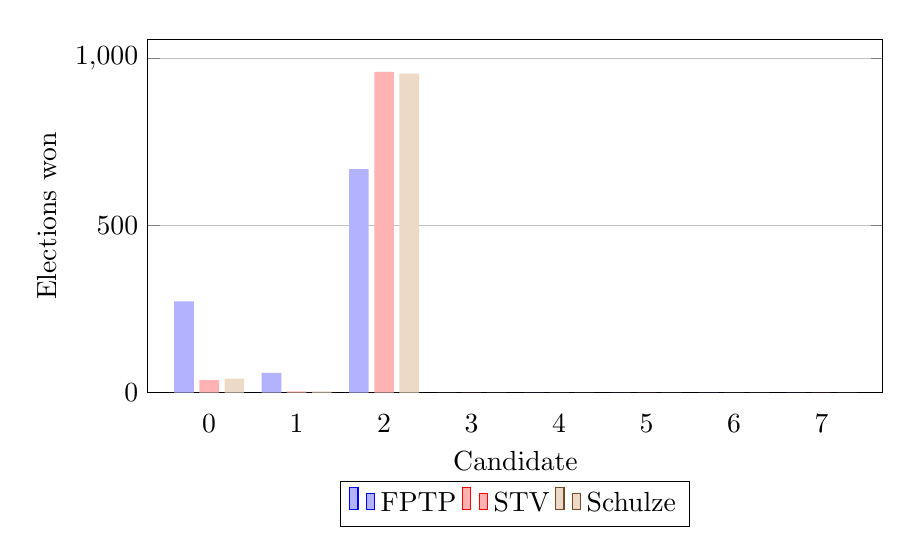
\begin{tikzpicture}
		\begin{axis}[
			ybar,
			width = 0.9\textwidth,
			height = 0.5\textwidth,
			legend style={at={(0.5,-0.25)},
			anchor=north,legend columns=-1},
      x tick style = transparent,
			ylabel = {Elections won},
			xlabel = {Candidate},
			ymajorgrids = true,
			every axis plot/.append style={draw=none,fill,no markers},
      ymin = 0,
			symbolic x coords={0,1,2,3,4,5,6,7,8},
			bar width=0.25cm
      ]
			\addplot coordinates
			{(0, 273)(1, 59)(2, 668)(3, 0)(4, 0)(5, 0)(6, 0)(7, 0)};
			\addplot coordinates
			{(0, 37)(1, 4)(2, 959)(3, 0)(4, 0)(5, 0)(6, 0)(7, 0)};
			\addplot coordinates
			{(0, 42)(1, 4)(2, 954)(3, 0)(4, 0)(5, 0)(6, 0)(7, 0)};
			\legend{FPTP, STV, Schulze}
		\end{axis}
	\end{tikzpicture}
	\caption{Results in scenario 1}
\label{fig:scenario 1 results}
\end{figure}

\begin{table}[H]
\centering
\caption{Key metrics for result in scenario 1}
\label{tab:scenario 1 result}
\begin{tabular}{@{}lccc@{}}
\toprule
Method & Standard deviation & Misrepresentation & Most likely winners \\ \midrule
FPTP & 223 & 66 & 2 \\
STV & 315 & 8 & 2 \\
Schulze & 313 & 9 & 2 \\ \bottomrule
\end{tabular}
\end{table}
% [ 223.39259164082, 315.44928276983, 313.6271671906]
\subsection{Scenario 2}
\label{sec:resuls-scenario2}
Scenario 2 featured nine candidates of which three were to be elected. The distribution of votes was ``normal'', and as seen in figure~\ref{fig:example of scenario 2} on page~\ref{fig:example of scenario 2}, the election is very close with many candidates having a similar percentage of first-preference votes. The results obtained in scenario 2 are very interesting. FPTP tended to underrepresent candidate 1, and elected a candidate from ideology 2 only in 28\% of elections, despite the ideology theoretically having 30\% of popular support. The Schulze method also tended to underrepresent ideology 2. It instead overrepresented ideology 3, electing 3 candidates of ideology 3 in 50\% of elections. This indicates that the Schulze method is not a representative method in a multi-seat election. The STV result showed less misrepresentation than the FPTP result, which was to be expected since the method has access to more data of any voter's preferences. The results in scenario 2 can be observed in figure~\ref{fig:scenario 2 result} and the key metrics can be seen in table~\ref{tab:scenario 2 result}.
\begin{figure}[H]
	\centering
	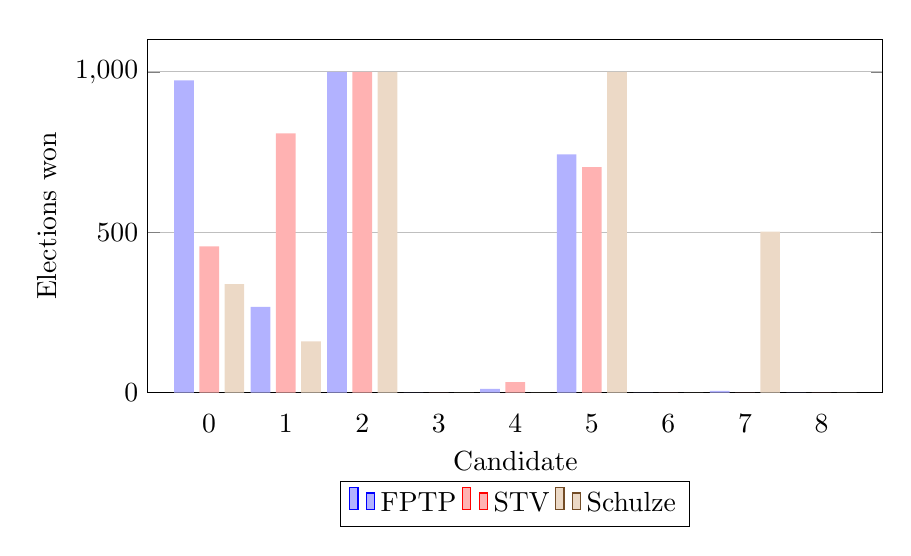
\begin{tikzpicture}
		\begin{axis}[
			ybar,
			width = 0.9\textwidth,
			height = 0.5\textwidth,
			legend style={at={(0.5,-0.25)},
			anchor=north,legend columns=-1},
      x tick style = transparent,
			ylabel = {Elections won},
			xlabel = {Candidate},
			ymajorgrids = true,
			every axis plot/.append style={draw=none,fill,no markers},
      ymin = 0,
			symbolic x coords={0,1,2,3,4,5,6,7,8},
			bar width=0.25cm
      ]
			\addplot coordinates
			{(0, 973)(1, 267)(2, 1000)(3, 0)(4, 12)(5, 743)(6, 0)(7, 5)(8, 0)};
			\addplot coordinates
			{(0, 456)(1, 808)(2, 1000)(3, 0)(4, 33)(5, 703)(6, 0)(7, 0)(8, 0)};
			\addplot coordinates
			{(0, 338)(1, 160)(2, 1000)(3, 0)(4, 0)(5, 1000)(6, 0)(7, 502)(8, 0)};
			\legend{FPTP, STV, Schulze}
		\end{axis}
	\end{tikzpicture}
	\caption{Results in scenario 2}
\label{fig:scenario 2 result}
\end{figure}

\begin{table}[H]
\centering
\caption{Key metrics for result in scenario 2}
\label{tab:scenario 2 result}
\begin{tabular}{@{}lccc@{}}
\toprule
Method & Standard deviation & Misrepresentation & Most likely winners \\ \midrule
FPTP & 418 & 50 & 0, 2 \& 5 \\
STV & 388 & 47 & 1, 2 \& 5 \\
Schulze & 393 & 100 & 2, 5 \& 7  \\ \bottomrule
\end{tabular}
\end{table}
% [ 418.13628234977, 388.17206952015, 393.25535950293 ]
\subsection{Scenario 3}
\label{sec:resuls-scenario3}
Scenario 3 featured nine candidates of which three were to be elected. The distribution of votes was  ``steep''. This can be seen by the first-preference votes in figure~\ref{fig:example of scenario 3} on Page~\pageref{fig:example of scenario 3}. The results obtained with each method in this scenario are practically identical. From this, it can be inferred that the results of the methods converge as the preferences in a population become more clear. The results obtained in this scenario can be seen in figure~\ref{fig:scenario 3 result}. The key metrics can be found in table~\ref{tab:scenario 3 result}.
\begin{figure}[H]
	\centering
	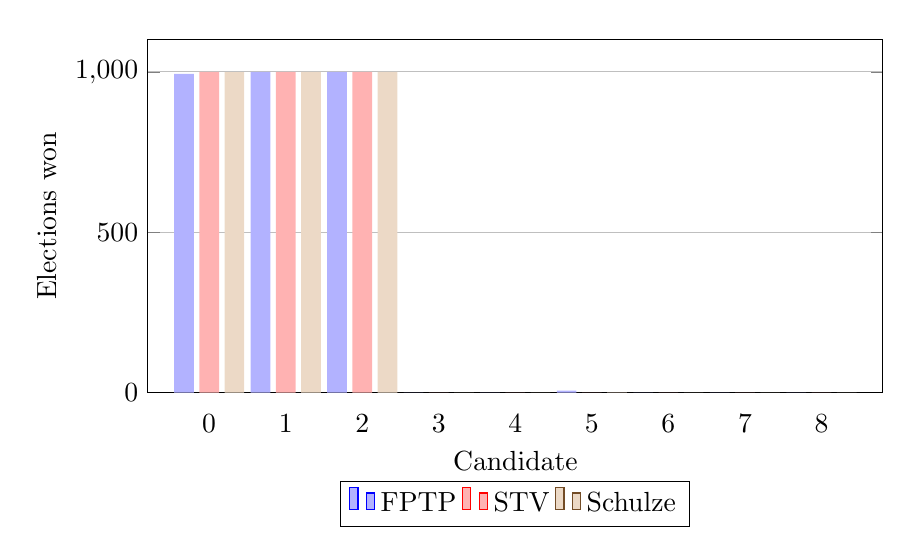
\begin{tikzpicture}
		\begin{axis}[
			ybar,
			width = 0.9\textwidth,
			height = 0.5\textwidth,
			legend style={at={(0.5,-0.25)},
			anchor=north,legend columns=-1},
      x tick style = transparent,
			ylabel = {Elections won},
			xlabel = {Candidate},
			ymajorgrids = true,
			every axis plot/.append style={draw=none,fill,no markers},
      ymin = 0,
			symbolic x coords={0,1,2,3,4,5,6,7,8},
			bar width=0.25cm
      ]
			\addplot coordinates
			{(0, 994)(1, 1000)(2, 1000)(3, 0)(4, 0)(5, 6)(6, 0)(7, 0)(8, 0)};
			\addplot coordinates
			{(0, 1000)(1, 1000)(2, 1000)(3, 0)(4, 0)(5, 0)(6, 0)(7, 0)(8, 0)};
			\addplot coordinates
			{(0, 999)(1, 1000)(2, 1000)(3, 0)(4, 0)(5, 1)(6, 0)(7, 0)(8, 0)};
			\legend{FPTP, STV, Schulze}
			\end{axis}
	\end{tikzpicture}
	\caption{Results in scenario 3}
\label{fig:scenario 3 result}
\end{figure}

\begin{table}[H]
	\centering
	\caption{Key metrics for result in scenario 3}
\label{tab:scenario 3 result}
	\begin{tabular}{@{}lccc@{}}
		\toprule
		Method & Standard deviation & Misrepresentation & Most likely winners \\ \midrule
		FPTP & 470 & 0 & 0, 1 \& 2 \\
		STV & 471 & 0 & 0, 1 \& 2 \\
		Schulze & 471 & 0 & 0, 1 \& 2  \\ \bottomrule
	\end{tabular}
\end{table}
\section{Conclusion}
The results obtained in the three different scenarios provide some insight into the varying properties of the different voting systems. Each of the methods showed different behavior in the different scenarios. For instance, the methods provided practically the same result in scenario 3 but wildly varying results in scenario 2. While the testing method used in this paper may not have been the most robust way of comparing the voting methods, several conclusions can be drawn from the data. They are outlined in 4 points below.
\begin{enumerate}
	\item Schulze did not seem to be a proportional voting method in multi-seat elections.\label{num:conclusion-schulze}
	
	As seen from the results obtained in scenario 2, which can be seen in Section~\ref{sec:resuls-scenario2}, the Schulze Method heavily overrepresented candidates from ideology 1 (candidates 3, 5 \& 7). While ideology 1 in fact was the most popular ideology, a more proportionate way of representing the electorate in the scenario would have been to grant one seat to each ideology. The Schulze tended to elect candidates from the strongest ideology only, instead of electing candidates from all ideologies in a more proportionate manner. This is not a problem in a single-seat election, as can be seen in the results of scenario 1 in Section~\ref{sec:resuls-scenario1}, which was a single-seat elections, where the Schulze Method simply elected the most popular candidate.
	\item In single-seat elections, Schulze and STV (and IRV in extension) seemed to provide similar results. 
	
	As seen in the results of scenario 1 outlined in Section~\ref{sec:resuls-scenario1}, both Schulze and STV produced nearly identical results, while the results from FPTP deviated slightly. While the methods work very differently, the results in these methods seem to behave similarly in single-seat elections.
	\item FPTP did not seem to be a very proportional method in close elections. 

	FPTP preformed considerably worse at being representative than the other methods. This was true for both close single- and multi-seat elections, excluding The Schulze Method in scenario 2 (see Point~\ref{num:conclusion-schulze}). At the core, both the STV and Schulze Method have more data to use for determining winners than what FPTP does. The FPTP method only has access to first-preference votes which does not convey as much information as a ballot listing all candidates in order of preference does.
	\item STV seems to be the most proportional method out of the 3 tested, but is not without its flaws.

	STV provided the most proportionate results overall of all three methods tested. However, as it goes with voting system, it has several flaws. It is for example possible to increase the chance of a candidate winning by lowering him/her on a ballot, and vice versa. STV is the only multi-seat proportional voting system tested in this paper, and the results obtained reinforce its position as just that.
\end{enumerate}
While there is no perfect voting system, they all preform differently. From the conclusions outlined above, a decision can be taken about what system analyzed in this paper to be used. Generally, if a proportional representation is desired (which in a democracy it usually is), STV will likely be the most appropriate method to use. In single-seat elections, the Schulze Method should also be considered. FPTP is the simplest method to both use and understand, but cannot be considered a proportionate voting method.

While the findings of this paper are hardly revolutionary, the nature of the three voting systems explored in this paper and their behavior is experimentally evaluated. The paper also provides implementations of all voting methods in both Typescript and JavaScript.

The key area for furthering this work would be in data collection or creation. A more sophisticated procedure for generating test data could be developed and run with more extensive test scenarios. Data from the real world could also be collected in actual elections and run through the different algorithms to test them. One could also write software that generates lots of scenarios with different parameters and analyzes how they differ automatically. Since the source code for this paper is open sourced under the MIT License, anyone can freely copy, modify and build on this work. This also makes for an open and transparent voting method where every voter can audit the system in use.
\pagebreak

\printbibliography{}
\pagebreak
\begin{appendices}
\section{Code implementation}
\begin{figure}[H]
\dirtree{%
.1 /.
.2 fptp/.
.3 index.ts.
.2 generator/.
.3 ballots.ts.
.3 index.ts.
.3 candidates.ts.
.3 interfaces.ts.
.2 schulze/.
.3 index.ts.
.2 stv/.
.3 candidate.ts.
.3 tree.ts.
.3 election.ts.
.3 index.ts.
.2 .gitignore.
.2 LICENSE.txt.
.2 package.json.
.2 README.md.
.2 tsconfig.json.
.2 tslint.json.
}
\caption{Project structure}
\label{fig:project-structure}
\end{figure}
The full source code for this project can be found at \url{https://github.com/adriansalamon/gymnasiearbete} and is open sourced under the MIT License. In order to run any of the implementations, the Typescript files (\Code{.ts}) need to be compiled to JavaScript files (\Code{.js}) using the Typescript Compiler. Then the code can be executed using Node.js. Code Example \ref{lst:project-example} shows an example of how to run an election.
\codeblock{code/projectExample.ts}{lst:project-example}{Example of how to run a Schulze Election with the code.}
All source code is commented and includes extensive use type annotations to help with orientation. The full project structure can be seen in Figure~\ref{fig:project-structure}.


\end{appendices}


\end{document}
